\documentclass[aspectratio=1610]{beamer}


% 主题选择
\usetheme{focus}
\usepackage{fontspec}
\usepackage{xeCJK}

\setmainfont{Fira Sans}  % 英文主字体
\setCJKmainfont{Microsoft YaHei}  % 中文主字体(系统中必须安装此字体)


\definecolor{main}{RGB}{0, 80, 60}
\definecolor{background}{RGB}{255, 255, 255}




\newcommand{\vuwlogo}{%
    \begin{tikzpicture}[remember picture,overlay]
    \node[anchor=north east,yshift=3.5pt,xshift=0pt] at (current page.north east) {\includegraphics[height=0.95cm]{figures/vuw.png}};
    \node[anchor=north east,yshift=3.5pt,xshift=-70pt] at (current page.north east) {\includegraphics[height=0.95cm]{figures/evostar2025.png}};
    \end{tikzpicture}%
}


\setbeamertemplate{navigation symbols}{}
\setbeamertemplate{footline}[frame number]


% 包
\usepackage{amsmath}
\usepackage{amssymb}
\usepackage{graphicx}
\usepackage{booktabs}
\usepackage{algorithm}
\usepackage{algpseudocode}
\usepackage{tikz}
\usepackage{CJKutf8}
\usetikzlibrary{shapes,arrows,positioning}

% Bib文件支持
\usepackage[backend=biber]{biblatex}
\usepackage{perpage}
\MakePerPage{footnote}
\addbibresource{example.bib}

\renewcommand*{\bibfont}{\normalfont\tiny}
\DeclareFieldFormat{beamercolorauthor}{%
    \usebeamercolor[fg]{bibliography entry author}%
    #1}
\DeclareFieldFormat{beamercolortitle}{%
    \usebeamercolor[fg]{bibliography entry title}%
    #1}
\DeclareFieldFormat{beamercolornote}{%
    \usebeamercolor[fg]{bibliography entry note}%
    #1}

\DeclareCiteCommand{\ajycite}
{\usebibmacro{prenote}}
{\printtext[beamercolorauthor]{%
    \printnames[given-family]{labelname}%
    \setunit{\addcomma\space}}%
\printtext[beamercolornote]{%
    \iffieldundef{journaltitle}
    {\printfield{booktitle}}  % Use booktitle if journaltitle is not present
    {\printfield{journaltitle}}%
    \setunit{\addspace}%
    \printtext[parens]{%
        \printdate}}}
{\multicitedelim}
{\usebibmacro{postnote}}


% 标题信息
\title[RAG-SR]{RAG-SR: 基于检索增强生成的神经符号回归}
\author[张等]{Hengzhe Zhang\textsuperscript{1}, Qi Chen\textsuperscript{1}, Bing Xue\textsuperscript{1}, Wolfgang Banzhaf\textsuperscript{2}, Mengjie Zhang\textsuperscript{1}}
\institute[惠灵顿维多利亚大学 & 密歇根州立大学]{
    \textsuperscript{1} 惠灵顿维多利亚大学工程与计算机科学学院
    \textsuperscript{2} 密歇根州立大学计算机科学与工程系
}
\date{ICLR 2025 (Spotlight)}


\begin{document}


% 标题页
    \begin{frame}
        \titlepage
    \end{frame}


% 大纲
    \begin{frame}{大纲}
        \tableofcontents
    \end{frame}


    \section{引言}

    \begin{frame}{符号回归}
        \begin{itemize}
            \item \textbf{符号回归(SR)}发现最能描述数据集的数学表达式
            \item 自动确定模型的\textbf{结构}$f$和\textbf{参数}$\theta$
            \item 提供\textbf{高精度}和\textbf{可解释性}
            \item 应用:物理学、生物学、金融、科学发现
        \end{itemize}

        \vspace{0.3cm}

        \textbf{数学定义:}
        \begin{align}
        (f^*, \theta^*)
            = \underset{f \in \mathcal{F}, \theta}{\text{argmin}} \sum_{i=1}^n \mathcal{L}(f(x_i, \theta), y_i)
        \end{align}
    \end{frame}

    \begin{frame}{问题定义:特征构建方法}
        \begin{itemize}
            \item 从数据集$(X, Y)$生成一组符号树/特征$\Phi = \{\phi_1, \ldots, \phi_m\}$
            \item 增强可解释模型$\mathcal{M}$(如线性回归)
            \item 目标:最小化损失函数
        \end{itemize}

        \begin{equation}
            \mathcal{L}(\Phi; X, Y) = \frac{1}{N} \sum_{i=1}^{N} \ell\left(\mathcal{M}\left(\phi_1(X_i), \ldots, \phi_m(X_i)\right), Y_i\right)
        \end{equation}

        \vspace{0.3cm}
        \textbf{优势:}
        \begin{itemize}
            \item 有效解决复杂的现实问题
            \item 多个弱特征可以共同发挥良好作用
        \end{itemize}
    \end{frame}


    \begin{frame}{当前方法的局限性:预训练模型}

        \begin{center}
            \textbf{预训练模型~\footnote{\ajycite{kamienny2022end}}}
            \begin{itemize}
                \item 仅限于已见函数
                \item 难以处理新变量
                \item 需要大规模预训练
            \end{itemize}
            \includegraphics[width=0.7\textwidth]{figs/E2E.png}
        \end{center}
    \end{frame}

    \begin{frame}{当前方法的局限性:强化学习}

        \begin{center}
            \textbf{强化学习~\footnote{\ajycite{landajuela2022unified}}}
            \begin{itemize}
                \item 样本效率低
                \item 反馈有限
                \item 收敛缓慢
            \end{itemize}
            \includegraphics[width=0.7\textwidth]{figs/DSR.png}
        \end{center}
    \end{frame}

    \begin{frame}{当前方法的局限性:稀疏监督学习}

        \begin{center}
            \textbf{稀疏监督学习~\footnote{\ajycite{sahoo2018learning}}}
            \begin{itemize}
                \item 依赖启发式剪枝
                \item 产生可能较大的解决方案
                \item 需要可微分的激活函数
            \end{itemize}
            \includegraphics[width=0.7\textwidth]{figs/EQL.png}
        \end{center}
    \end{frame}


    \begin{frame}{相关工作}
        \begin{columns}
            \begin{column}{0.48\textwidth}
                \textbf{神经符号回归}
                \begin{itemize}
                    \item 预训练模型(DSR, E2E)难以处理未见函数/变量
                    \item 强化学习方法样本效率低
                    \item 稀疏监督学习需要可微分激活函数
                \end{itemize}
            \end{column}
            \begin{column}{0.48\textwidth}
                \textbf{进化符号回归}
                \begin{itemize}
                    \item 传统GP缺乏搜索有效性
                    \item 语义GP有效但仅依赖现有构建块
                    \item 进化过程中知识保留有限
                \end{itemize}
            \end{column}
        \end{columns}
    \end{frame}


    \begin{frame}{核心洞见:用良好解决方案指导神经生成}
        \begin{alertblock}{核心洞见}
            \textbf{从语言模型角度:}
            \begin{itemize}
                \item 直接使用神经网络改进解决方案会导致幻觉
                \item 更好的方法:向模型展示可能的改进,并要求它生成更好的方案
            \end{itemize}

            \textbf{从进化算法角度:}
            \begin{itemize}
                \item 不要问"给我一个好的变异",而是展示好的变异示例并说"好的变异是这样的,给我一个更好的"
            \end{itemize}

            \textbf{使用ChatGPT等大语言模型时:}
            \begin{itemize}
                \item 不要问:"当前程序只能做B,但我想要它做A"
                \item 而应该问:"当前程序只能做B,我想要它做A,我认为一个潜在的方向是..."
            \end{itemize}
        \end{alertblock}
    \end{frame}


    \begin{frame}{RAG-SR:一种新颖的语义到符号学习框架}
        \textbf{我们的方法:}通过在线学习将进化特征构建与神经网络集成

        \begin{itemize}
            \item \textbf{语义下降:}通过在线监督学习实时自适应生成与所需语义一致的符号树

            \item \textbf{检索增强生成:}通过利用库中的符号表达式减轻幻觉问题

            \item \textbf{掩码对比学习:}捕获语义等价但句法不同的符号表达式

            \item \textbf{尺度不变数据增强和双重查询策略:}提高对线性回归的鲁棒性
        \end{itemize}
    \end{frame}


    \section{方法论}

    \begin{frame}{RAG-SR:解决方案初始化与评估}
        \begin{columns}
            \begin{column}{0.5\textwidth}
                \textbf{步骤1:解决方案初始化}
                \begin{itemize}
                    \item 使用ramped half-and-half生成随机符号树
                \end{itemize}

                \vspace{0.3cm}
                \textbf{步骤2:解决方案评估}
                \begin{itemize}
                    \item 通过留一交叉验证的岭回归评估特征
                \end{itemize}
            \end{column}
            \begin{column}{0.5\textwidth}
                \includegraphics[width=1.0\textwidth]{figs/Workflow.pdf}
            \end{column}
        \end{columns}
    \end{frame}

    \begin{frame}{RAG-SR:语义库构建}
        \begin{columns}
            \begin{column}{0.5\textwidth}
                \textbf{步骤3:语义库构建}
                \begin{itemize}
                    \item \textbf{检索库:}具有KD树的FIFO队列,用于高效检索
                    \begin{itemize}
                        \item 由于特征构建对尺度不敏感,语义在存储前会被归一化
                    \end{itemize}
                    \item \textbf{神经语义库:}使用检索库中的配对进行训练
                \end{itemize}
            \end{column}
            \begin{column}{0.5\textwidth}
                \includegraphics[width=1.0\textwidth]{figs/Workflow.pdf}
            \end{column}
        \end{columns}
    \end{frame}

    \begin{frame}{RAG-SR:解决方案选择过程}
        \begin{columns}
            \begin{column}{0.5\textwidth}
                \textbf{步骤4:解决方案选择}
                \begin{itemize}
                    \item 使用Lexicase selection选择有前景的父代
                \end{itemize}
            \end{column}
            \begin{column}{0.5\textwidth}
                \includegraphics[width=1.0\textwidth]{figs/Workflow.pdf}
            \end{column}
        \end{columns}
    \end{frame}

    \begin{frame}{RAG-SR:解决方案生成}
        \begin{columns}
            \begin{column}{0.5\textwidth}
                \textbf{步骤5:解决方案生成}
                \begin{itemize}
                    \item \textbf{语义下降:}局部搜索以改进解决方案
                    \item \textbf{进化搜索:}使用GP算子进行全局探索
                \end{itemize}
            \end{column}
            \begin{column}{0.5\textwidth}
                \includegraphics[width=1.0\textwidth]{figs/Workflow.pdf}
            \end{column}
        \end{columns}
    \end{frame}

    \begin{frame}{RAG-SR:档案维护}
        \begin{columns}
            \begin{column}{0.5\textwidth}
                \textbf{步骤6:档案维护}
                \begin{itemize}
                    \item 存储表现最佳的解决方案
                \end{itemize}
            \end{column}
            \begin{column}{0.5\textwidth}
                \includegraphics[width=1.0\textwidth]{figs/Workflow.pdf}
            \end{column}
        \end{columns}
    \end{frame}

    \begin{frame}{语义下降:概述}
        % 图片放在上方
        \begin{center}
            \includegraphics[width=0.75\textwidth, trim=8pt 8pt 8pt 8pt, clip]{figs/Motivation.pdf}
        \end{center}

        % 文字放在下方
        \textbf{关键原则:}
        \begin{itemize}
            \item 迭代优化替换次优特征,同时保持特征数量恒定
        \end{itemize}
    \end{frame}

    \begin{frame}{语义下降:步骤1-2}
        % 图片放在上方
        \begin{center}
            \includegraphics[width=0.75\textwidth, trim=8pt 8pt 8pt 8pt, clip]{figs/Motivation.pdf}
        \end{center}

        % 文字放在下方
        \textbf{对解决方案$\{\phi_1, \ldots, \phi_m\}$中的每棵树$\phi_i$:}
        \begin{enumerate}
            \item 暂时移除$\phi_i$的贡献:\\
            $\Phi^{temp}(X) = \Phi(X) - \beta_i \phi_i(X)$
            \item 计算残差$R = Y - \Phi^{temp}(X)$
        \end{enumerate}
    \end{frame}
    \begin{frame}{语义下降:步骤3}
        % 图片放在上方
        \begin{center}
            \includegraphics[width=0.75\textwidth, trim=8pt 8pt 8pt 8pt, clip]{figs/Motivation.pdf}
        \end{center}

        % 文字放在下方
        \textbf{使用以下方法生成新树填补这个空缺:}
        \begin{itemize}
            \item 以概率$P_{neural}$进行神经生成:"这是之前有效的模式,生成更好的"
            \item 以概率$1-P_{neural}$从语义库检索:"找到我们之前见过的最佳匹配模式"
        \end{itemize}
    \end{frame}

    \begin{frame}{语义下降:步骤4}
        % 图片放在上方
        \begin{center}
            \includegraphics[width=0.75\textwidth, trim=8pt 8pt 8pt 8pt, clip]{figs/Motivation.pdf}
        \end{center}

        % 文字放在下方
        \textbf{最后步骤:}
        \begin{itemize}
            \item 如果检索生成的新树减少了误差则接受,如果是神经生成则直接接受
            \item 对解决方案中的所有树迭代继续此过程
        \end{itemize}
    \end{frame}

    \begin{frame}{检索增强生成}
        % 图片在上方
        \begin{center}
            \includegraphics[width=0.7\textwidth]{figs/NN.pdf}
        \end{center}

        % 文字在下方
        \textbf{挑战:}语言模型总能生成内容,但可能与给定任务无关

        \textbf{核心思想:}检索增强生成减少幻觉

        \begin{itemize}
            \item \textbf{数据收集:}在库中存储评估过的子树及其语义
            \item \textbf{网络训练:}将语义映射到符号表达式
            \item \textbf{检索:}从有前景的表达式提供上下文
        \end{itemize}
    \end{frame}

    \begin{frame}{神经网络架构}
        % 图片在上方
        \begin{center}
            \includegraphics[width=0.7\textwidth]{figs/NN.pdf}
        \end{center}

        % 文字在下方
        \begin{itemize}
            \item \textbf{带有残差连接的MLP:}处理所需语义$R$
            \item \textbf{Transformer编码器:}处理最近的符号树$\hat{\phi}$
            \item \textbf{Transformer解码器:}生成新树的标记序列
            \item \textbf{输出:}与$R$语义对齐的有效符号树$\phi$
        \end{itemize}
    \end{frame}



    \begin{frame}{损失函数}
        \textbf{双目标损失函数:}

        \begin{equation}
            \mathcal{L} = \mathcal{L}_{\text{cross-entropy}} + \lambda \cdot \mathcal{L}_{\text{InfoNCE}}
        \end{equation}

        \textbf{交叉熵损失:}序列生成的传统目标

        \textbf{InfoNCE损失:}捕获语义等价性的对比学习
    \end{frame}


    \begin{frame}{掩码对比损失}
        \textbf{目标:}对齐来自意图编码和检索增强编码的嵌入

        \vspace{0.2cm}
        \textbf{过程:}
        \begin{itemize}
            \item 最近语义$\hat{\phi}(X) \in \mathbb{R}^{B \times N}$ → MLP → $\mathbf{F}_{\text{nearest}} \in \mathbb{R}^{B \times K}$
            \item 符号嵌入$\mathbf{H}_{\text{Transformer}} \in \mathbb{R}^{B \times L \times D}$ → 平均 → $\mathbf{H}_{\text{avg}} \in \mathbb{R}^{B \times D}$
        \end{itemize}

        \vspace{0.2cm}
        \textbf{带掩码的InfoNCE损失:}
        \begin{equation}
            \mathcal{L}_{\text{InfoNCE}} = - \frac{1}{B} \sum_{i=1}^{B} \log \frac{\exp\left(\text{sim}(\mathbf{F}_{\text{nearest}}[i], \mathbf{H}_{\text{avg}}[i]) / \tau\right)}{\sum_{j=1}^{B} \exp\left(\text{sim}(\mathbf{F}_{\text{nearest}}[i], \mathbf{H}_{\text{avg}}[j]) \cdot \text{mask} / \tau\right)}
        \end{equation}


    \end{frame}


    \begin{frame}{对比学习的效果}
        \begin{columns}
            \begin{column}{0.55\textwidth}
                \begin{figure}
                    \centering
                    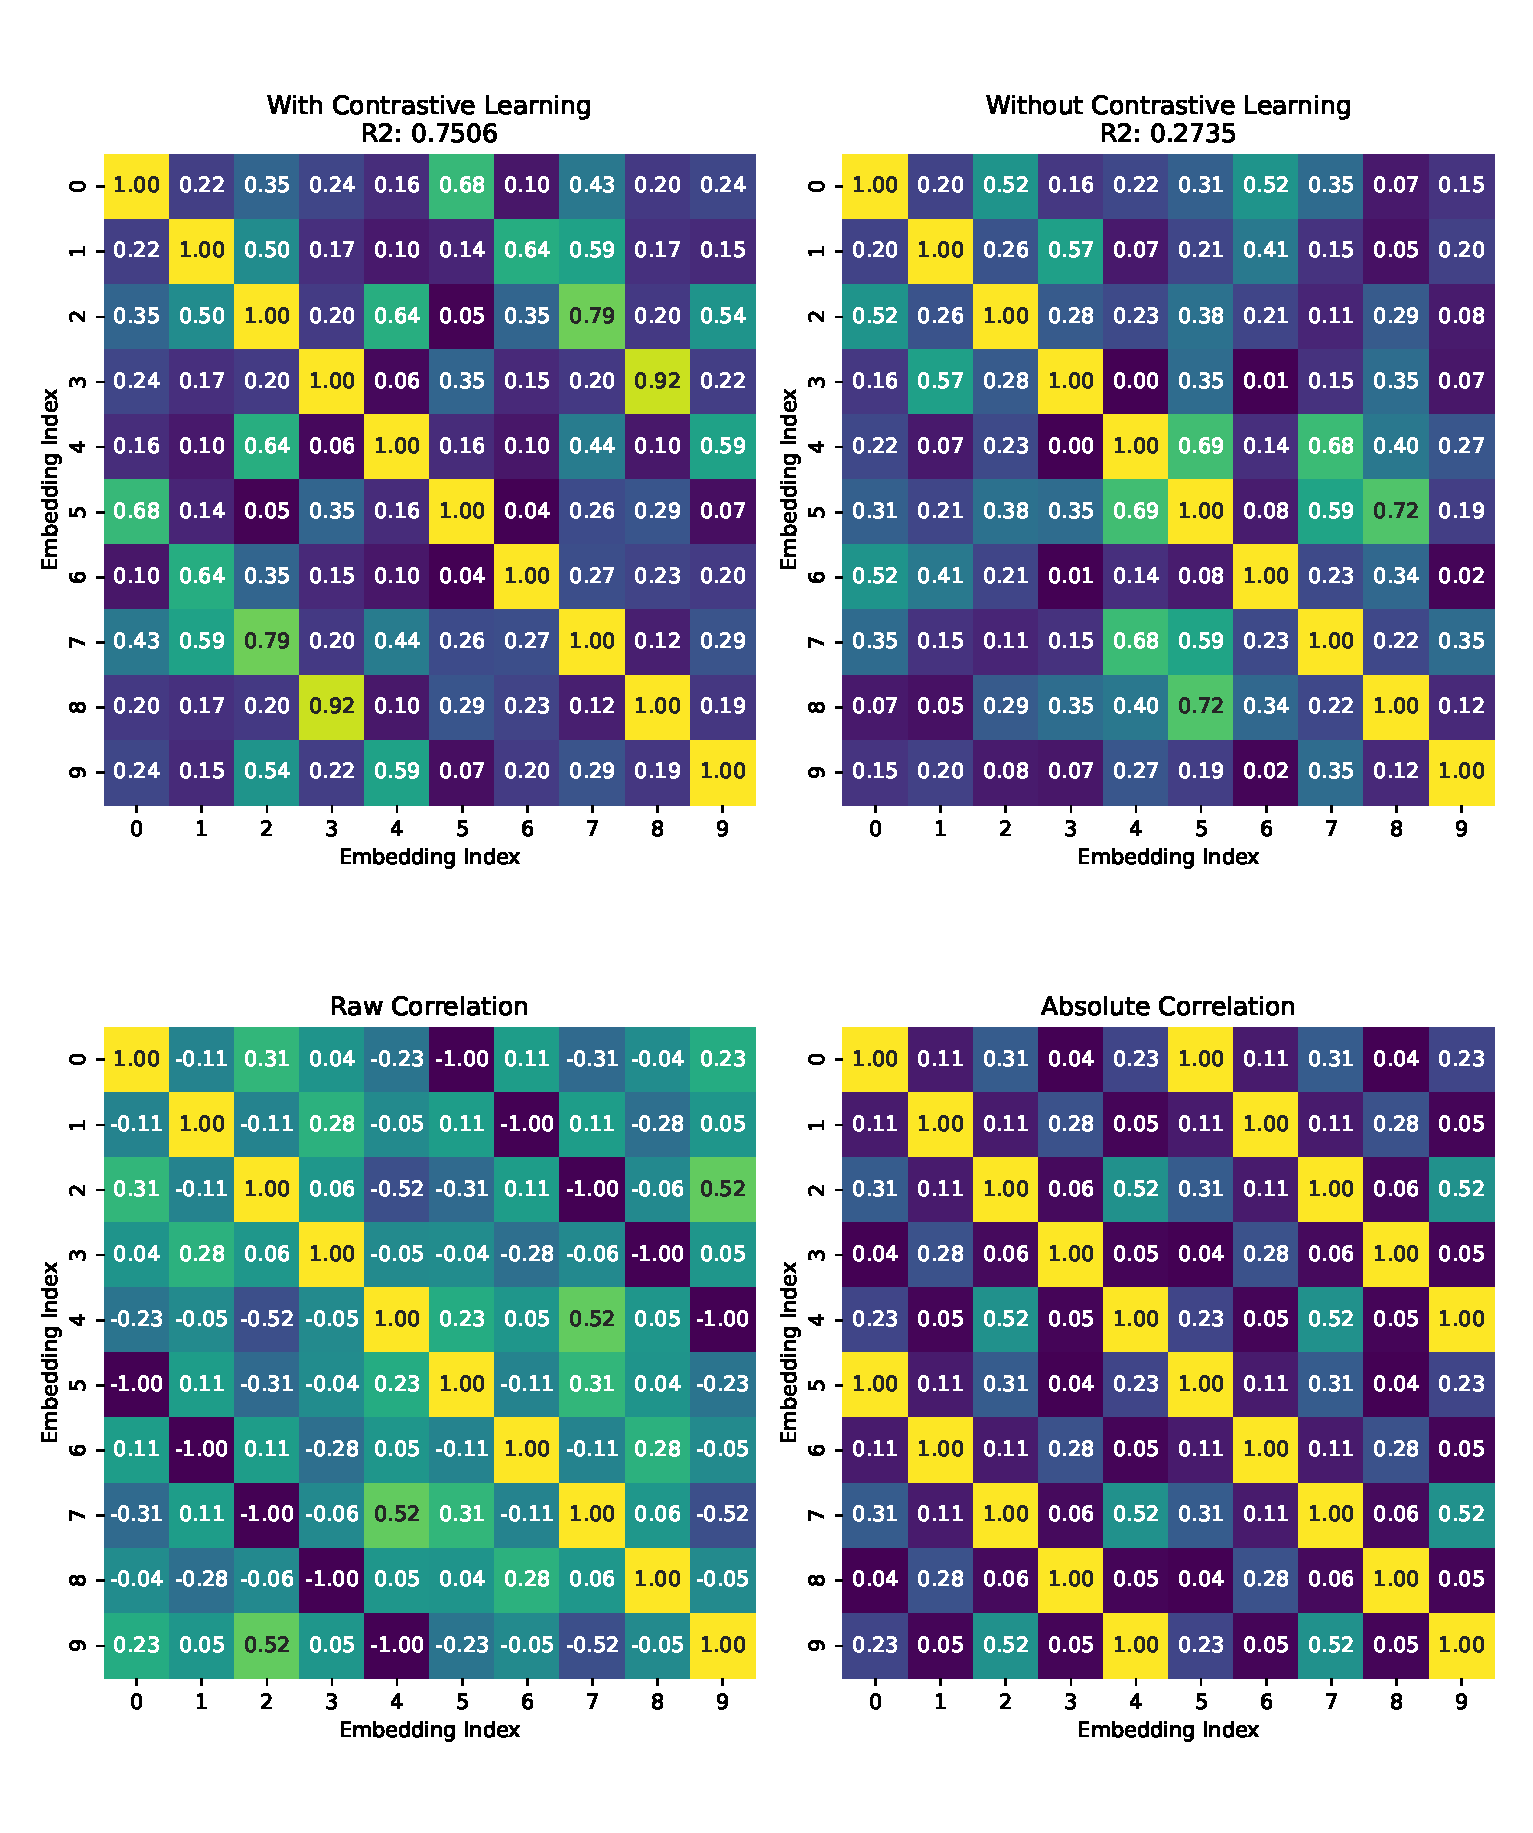
\includegraphics[height=0.8\textheight]{figs/data_augmentation_heatmap.eps}
                \end{figure}
            \end{column}

            \begin{column}{0.45\textwidth}
                \textbf{掩码策略:}
                \begin{itemize}
                    \item 掩码矩阵消除假负例(余弦相似度>0.99)
                    \item 防止对语义相似表达式进行惩罚
                    \item 提高对真正不同表达式的区分能力
                \end{itemize}

                \textbf{关键发现:}
                \vspace{0.3cm}
                \begin{itemize}
                    \item 捕获具有相同语义的不同表达式为等价
                    \vspace{0.2cm}
                    \item 没有它:等价语义会有不同嵌入
                    \vspace{0.2cm}
                \end{itemize}
            \end{column}
        \end{columns}
    \end{frame}

    \begin{frame}{数据增强与双重查询}
        \textbf{符号不变性:}在线性回归中,系数的符号会自动调整

        \textbf{数据增强:}包括原始特征对$(\psi, \psi(X))$及其取反$(\psi, -\psi(X))$
        \begin{equation}
            \mathcal{T} \gets \mathcal{T} \cup \{(\psi, -\psi(X)) \mid (\psi, \psi(X)) \in \mathcal{T}\}
        \end{equation}

        \textbf{双重查询:}
        \begin{itemize}
            \item 同时用所需语义$R$及其取反$-R$查询神经网络
            \item 生成候选树$\phi$和$\phi'$
            \item 选择概率最高的树
        \end{itemize}

    \end{frame}


    \section{实验}

    \begin{frame}{实验设置}
        \textbf{数据集:}
        \begin{itemize}
            \item PMLB基准测试中的120个黑盒数据集
            \item 119个费曼方程和14个Strogatz数据集
        \end{itemize}

        \textbf{评估方式:}
        \begin{itemize}
            \item 75:25训练-测试分割
            \item 10次重复以保证鲁棒性
            \item 测试集上的$R^2$分数作为评价指标
            \item 输入特征 Min-max scaling
        \end{itemize}

        \textbf{配置:}
        \begin{itemize}
            \item 种群大小:200
            \item 代数:100
            \item 每个解决方案包含10棵树
            \item $P_{neural} = 0.1$
        \end{itemize}
    \end{frame}

    \begin{frame}{组件评估:编辑距离}
        \begin{center}
            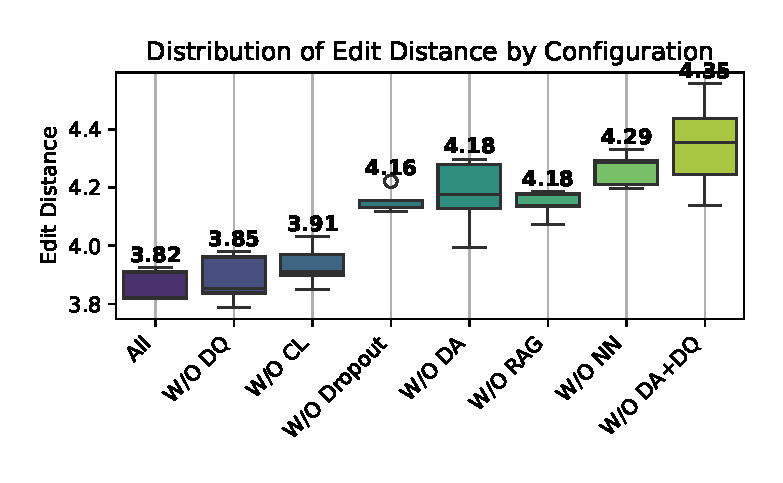
\includegraphics[width=0.6\textwidth]{figs/ablation_study_accuracy_10.eps}
        \end{center}

        \textbf{观察结果:}
        \begin{itemize}
            \item 神经生成的性能优于简单检索(W/O NN)
            \item 所有组件一起使用实现了最低的编辑距离
            \item RAG具有最显著的影响,其次是数据增强
            \item Dropout、对比学习和双重查询显示出适度的好处
        \end{itemize}
    \end{frame}

    \begin{frame}{组件评估:运行时间}
        \begin{center}
            \includegraphics[width=0.6\textwidth]{figs/ablation_study_time_10.eps}
        \end{center}

        \textbf{观察结果:}
        \begin{itemize}
            \item RAG适度增加了运行时间
            \item 移除DA和DQ减少了时间但牺牲了准确性
            \item 计算成本和性能之间的权衡
            \item 考虑到准确性提升,开销是可接受的
        \end{itemize}
    \end{frame}

    \begin{frame}{生成树示例}
        \begin{table}
            \centering
            \footnotesize
            \begin{tabular}{cc}
                \toprule
                RAG-NN生成的树(距离)           & 简单NN生成的树(距离)             \\
                \midrule
                Sin(Sin(ARG3)) (0)       & Cos(Cos(Cos(ARG9))) (4)  \\
                AQ(ARG7, ARG8) (0)       & Log(Max(ARG7, ARG7)) (3) \\
                Max(ARG1, ARG8) (0)      & Subtract(ARG1, ARG1) (2) \\
                Sqrt(Sqrt(ARG2)) (0)     & Log(Log(ARG2)) (2)       \\
                Subtract(ARG6, ARG7) (0) & Max(ARG7, ARG7) (2)      \\
                \bottomrule
            \end{tabular}
        \end{table}

        \begin{table}
            \centering
            \footnotesize
            \begin{tabular}{cc}
                \toprule
                检索树(距离)                                           & 真实树                  \\
                \midrule
                Sin(ARG3) (1)                                     & Sin(Sin(ARG3))       \\
                Log(Neg(Max(AQ(ARG8, ARG0), AQ(ARG7, ARG8)))) (6) & AQ(ARG7, ARG8)       \\
                Max(add(Abs(Sin(Cos(ARG6))), ARG8), ARG1) (6)     & Max(ARG1, ARG8)      \\
                Square(Log(ARG2)) (2)                             & Sqrt(Sqrt(ARG2))     \\
                Subtract(ARG7, ARG6) (2)                          & Subtract(ARG6, ARG7) \\
                \bottomrule
            \end{tabular}
        \end{table}

        \textbf{观察结果:}RAG显著提高了神经网络生成正确表达式的能力
    \end{frame}

    \begin{frame}{SR基准测试的表现}
        \begin{columns}
            \begin{column}{0.6\textwidth}
                \begin{center}
                    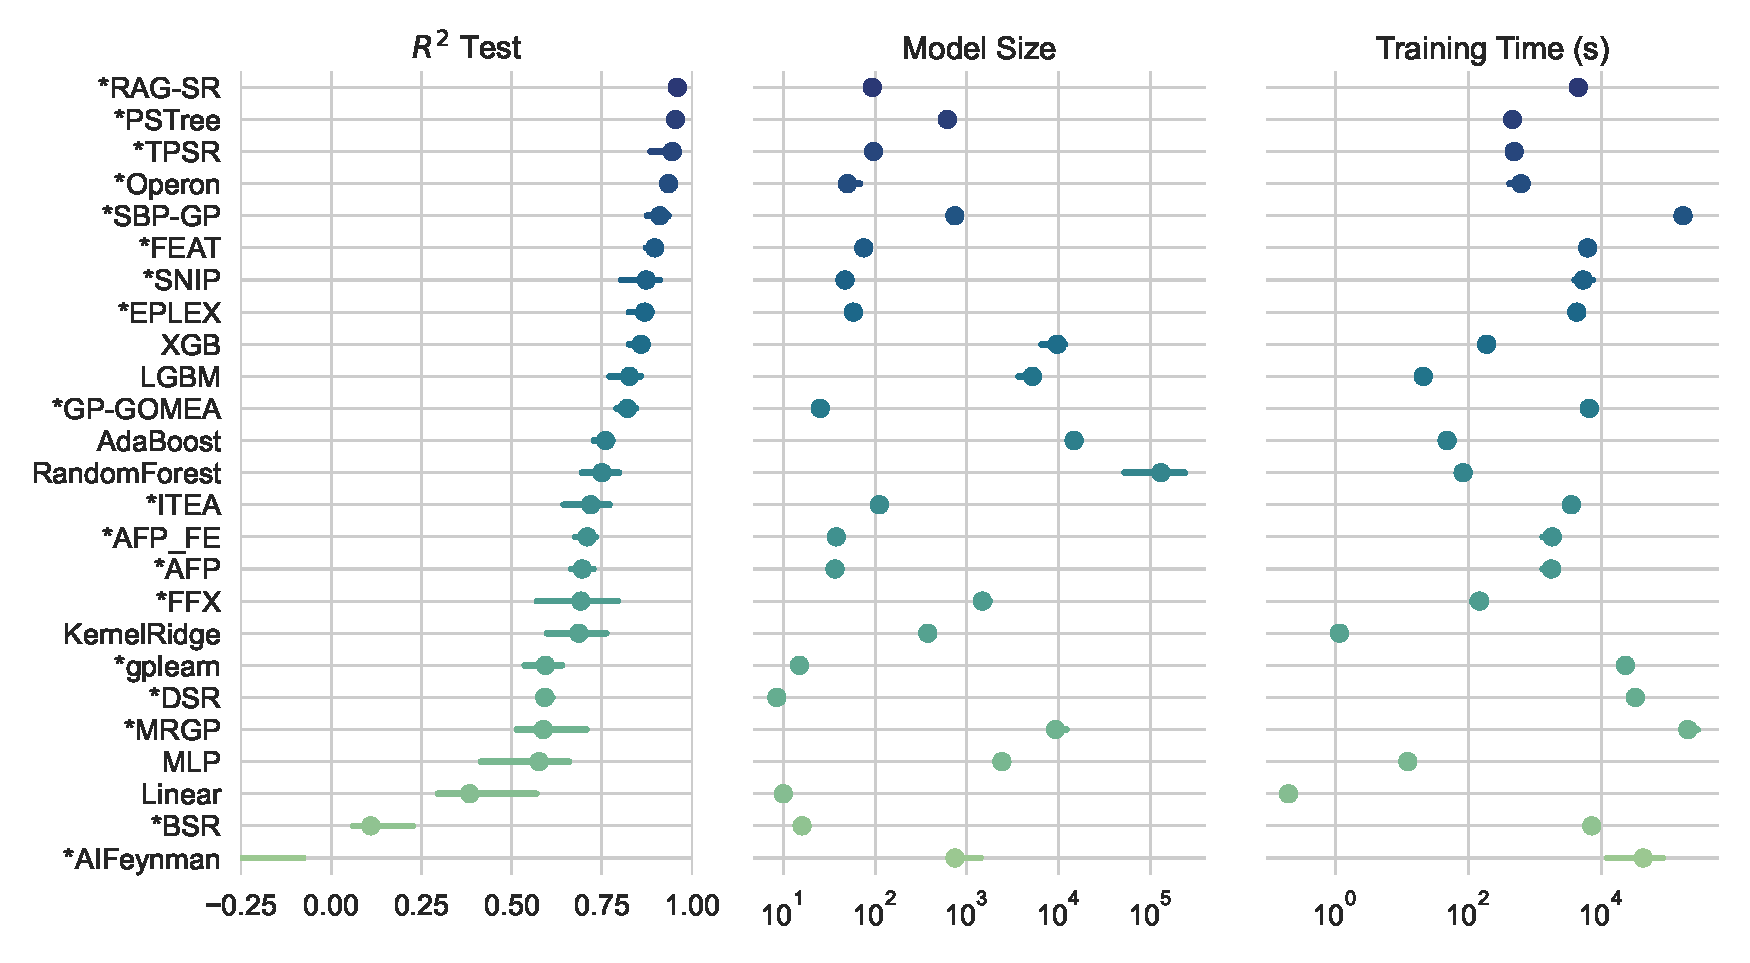
\includegraphics[width=\textwidth]{figs/pairgrid-pointplot_r2_test_model_size_training-time-(s).eps}
                \end{center}
            \end{column}

            \begin{column}{0.38\textwidth}
                \textbf{观察结果:}
                \begin{itemize}
                    \item RAG-SR在$R^2$分数上优于所有25种算法
                    \item 生成的模型比SBP-GP小一个数量级
                    \item 训练时间与FEAT相当
                    \item 准确性、复杂性和效率之间的最佳平衡
                \end{itemize}
            \end{column}
        \end{columns}
    \end{frame}

    \begin{frame}{统计显著性}
        \begin{columns}
            \begin{column}{0.48\textwidth}
                \begin{center}
                    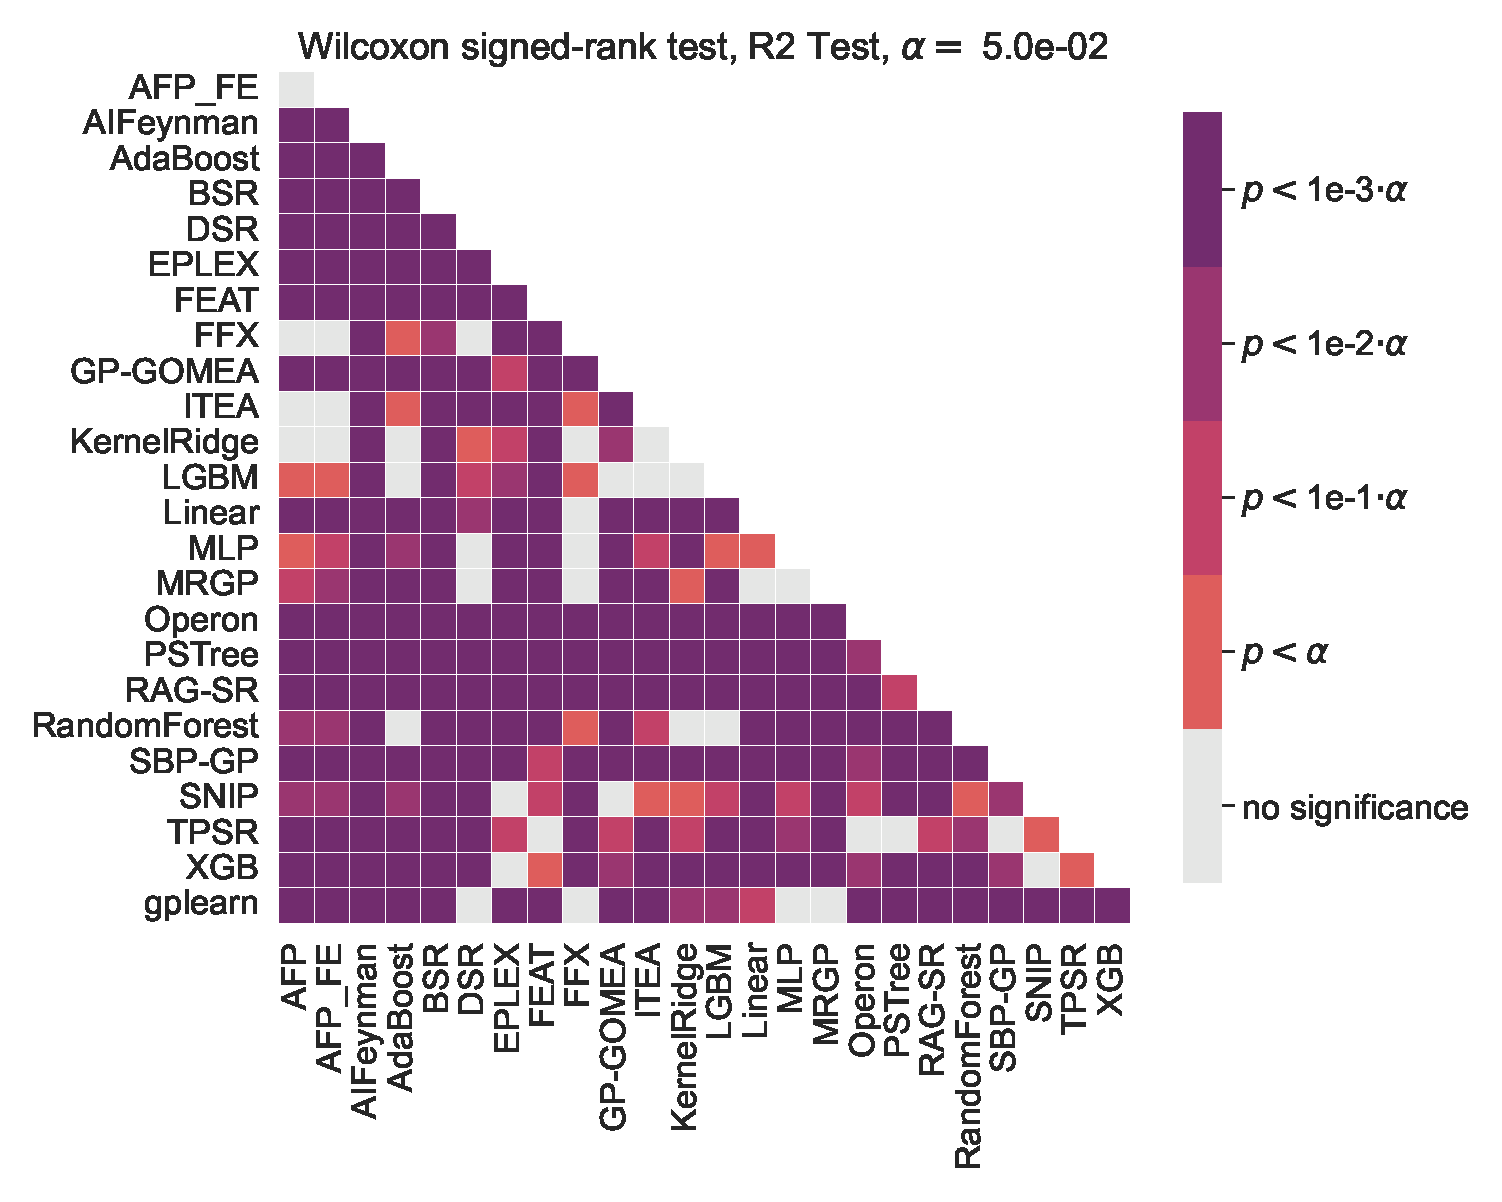
\includegraphics[width=\textwidth]{figs/Pairwise_comparison_of_R2_Test_on_black-box_problems.eps}
                \end{center}
            \end{column}

            \begin{column}{0.48\textwidth}
                \textbf{观察结果:}
                \begin{itemize}
                    \item RAG-SR显著优于所有其他方法
                    \item 相对于TPSR的改进证实了在线学习相比预训练的有效性
                    \item 相对于SBP-GP的优势表明集成神经网络组件的价值
                \end{itemize}
            \end{column}
        \end{columns}
    \end{frame}

    \begin{frame}{帕累托前沿分析}
        \begin{columns}
            \begin{column}{0.48\textwidth}
                \begin{center}
                    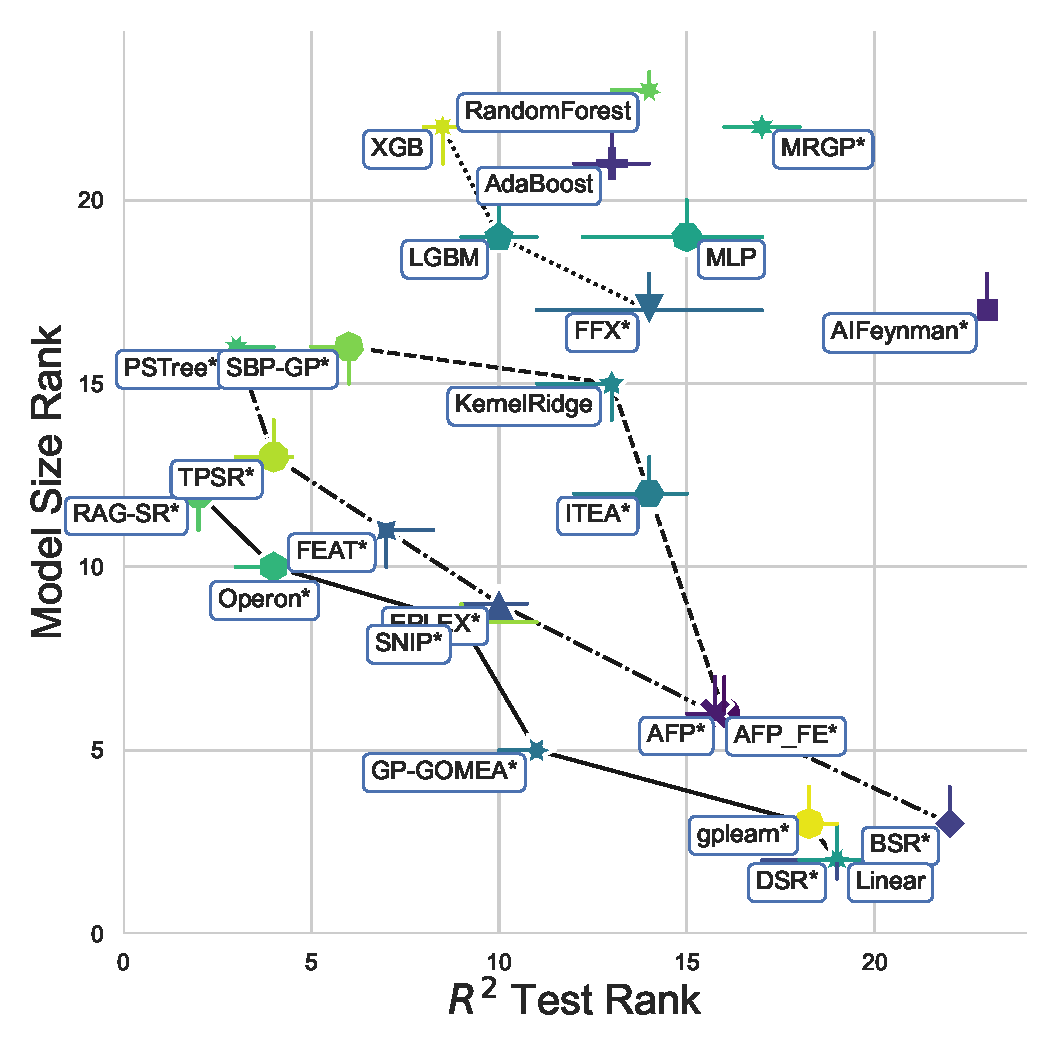
\includegraphics[width=\textwidth]{figs/pareto_plot_r2_test_rank_model_size_rank.eps}
                \end{center}
            \end{column}

            \begin{column}{0.48\textwidth}
                \textbf{观察结果:}
                \begin{itemize}
                    \item RAG-SR出现在第一帕累托前沿
                    \item 准确性和模型复杂性之间的优异平衡
                \end{itemize}
            \end{column}
        \end{columns}
    \end{frame}

    \begin{frame}{费曼和Strogatz结果}
        \begin{center}
            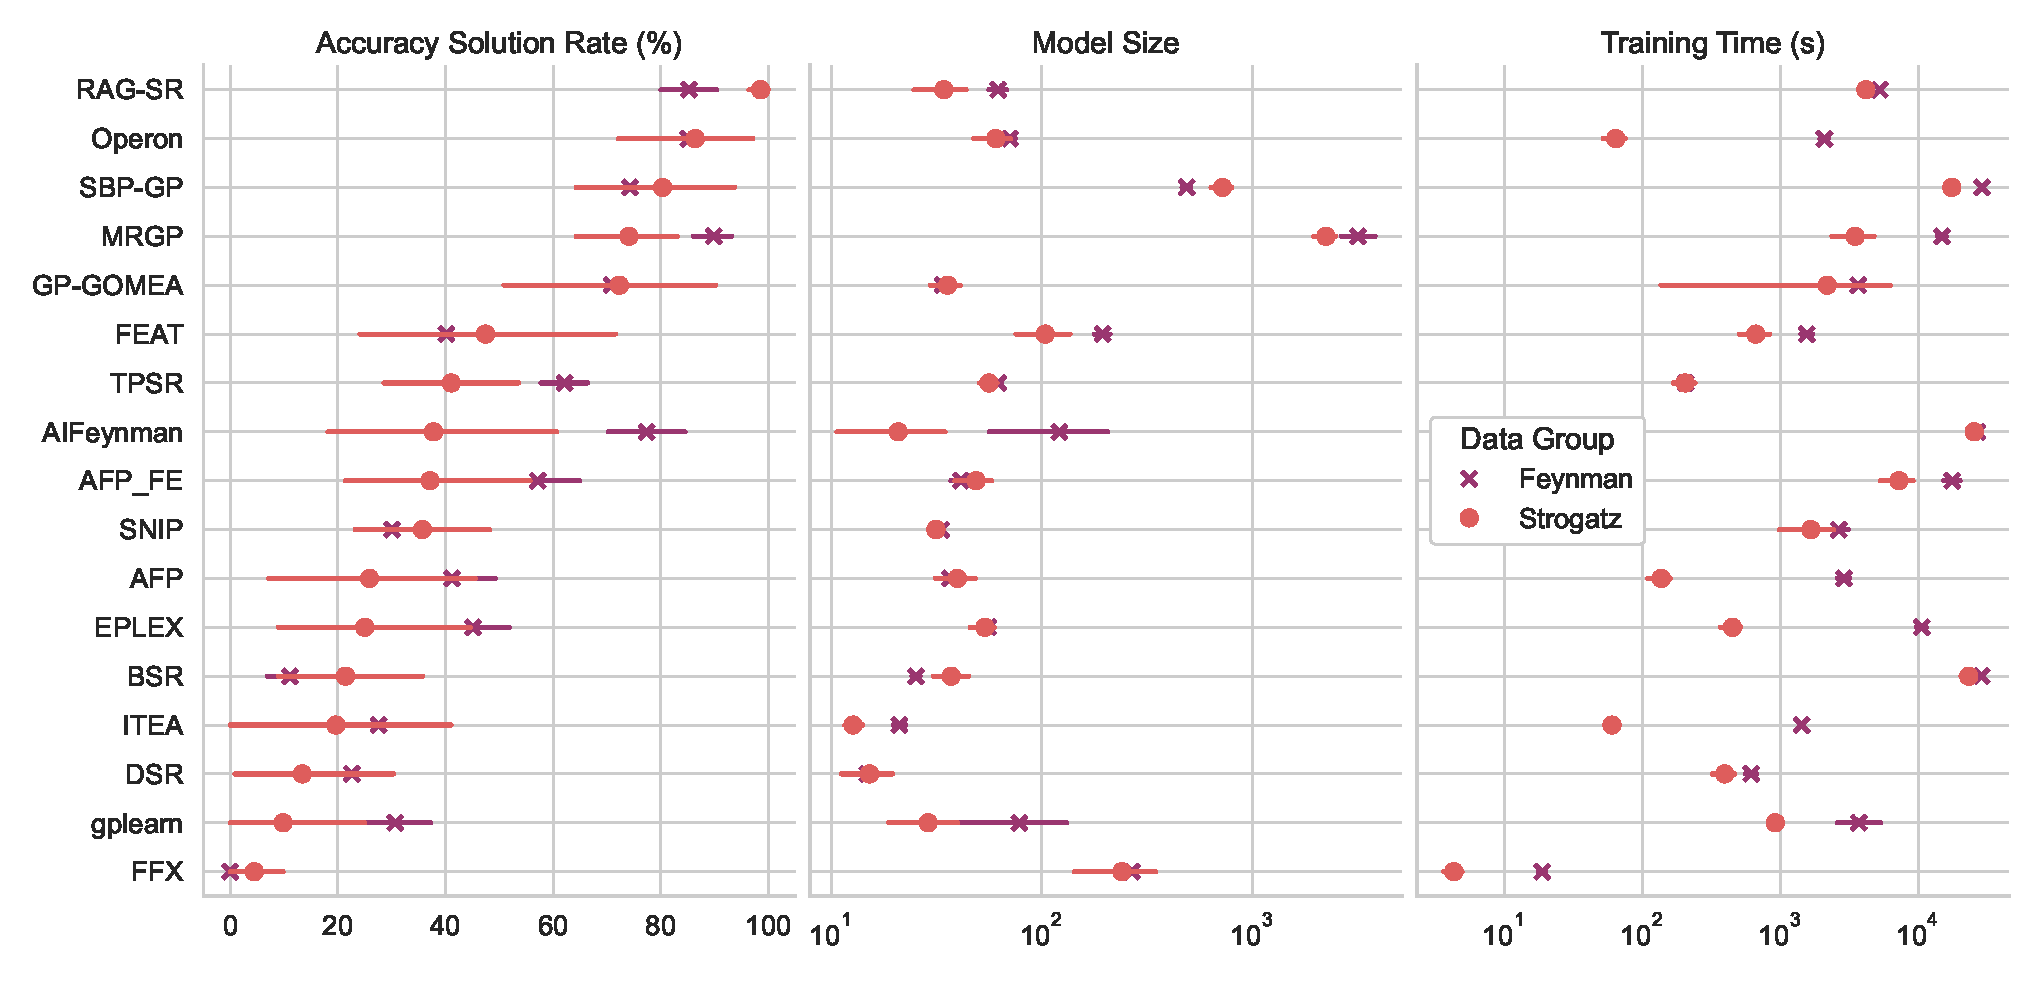
\includegraphics[width=0.8\textwidth]{figs/pairgrid_accuracy_solution_rate_(pct)_model_size_training-time-(s).eps}
        \end{center}

        \textbf{观察结果:}
        \begin{itemize}
            \item Strogatz数据集上的测试$R^2$分数最高
            \item 费曼数据集上排名第二(仅次于MRGP)
            \item MRGP模型大一个数量级
            \item 显著优于基于深度学习的SR方法
        \end{itemize}
    \end{frame}


    \section{结论}

    \begin{frame}{结论}
        \textbf{贡献:}
        \begin{itemize}
            \item 具有检索增强神经语义库的新型符号回归方法
            \item 无需预训练的有效在线学习方法
            \item 有效减轻幻觉的检索增强方法
            \item 考虑语义等价性的对比学习,提高有效性
            \item 利用符号不变性的数据增强和双重查询,提升性能
        \end{itemize}

        \textbf{未来方向:}
        \begin{itemize}
            \item 扩展到有限样本的噪声数据集
            \item GPU加速结合预训练和在线学习
        \end{itemize}
    \end{frame}

    \begin{frame}{关键要点}
        \begin{center}
            \Large
            \alert{RAG-SR的关键创新:}

            \vspace{0.5cm}

            \begin{beamercolorbox}[rounded=true,shadow=true,sep=1em]{block body}
                不要要求神经网络直接生成好的改进。\\
                \vspace{0.3cm}
                相反,展示好的改进例子并说:\\
                ``好的改进是这样的,现在给我一个更好的。''
            \end{beamercolorbox}
        \end{center}
    \end{frame}

    \begin{frame}{}
        \begin{center}
            \Large{\textbf{谢谢!}}

            \vspace{1cm}

            \normalsize
            源代码:\url{https://github.com/hengzhe-zhang/RAG-SR}
        \end{center}
    \end{frame}

\end{document}

